\chapter{Fundamentação teórica}
\label{cap:fundamentacao}

\section{Hierarquia de memória}
A hierarquização da cache em múltiplos níveis é uma solução para aumentar o desempenho no funcionamento das memórias caches. O nível de cache mais alto é chamado de L1 (\textit{Level 1}), com baixa capacidade de armazenamento e com altíssima velocidade de acesso. O segundo nível, L2 (\textit{Level 2}), possui maior capacidade de armazenamento, porém com velocidade de acesso inferior a L1. Quando a UCP necessita acessar um dado na memória principal, primeiramente é verificado se o dado encontra-se na cache L1. Caso o dado seja encontrado, obtém-se um excelente desempenho no acesso à informação, porém, caso o dado não seja encontrado, a busca prossegue para a L2.

Um processador pode ser projetado com diversos níveis de cache, conforme especificação do fabricante. Como exemplos, o processador da Motorola Power PC G4 possui cache de nível 2, enquanto o processador Intel Xeon MP possui cache de nível 3 \cite{machado2013}.

\section{Princípio da localidade}
O \textit{caching} talvez seja o exemplo mais importante da grande ideia da predição. Ele conta com o princípio da localidade para tentar encontrar os dados desejados nos níveis mais altos da hierarquia de memória, e oferece mecanismos para garantir que, quando a predição for errada, ela encontra e usa os dados apropriados dos níveis mais baixos da hierarquia da memória. As taxas de acerto da predição de cache nos computadores modernos, normalmente, são mais altas do que 95\% \cite{patterson2017}.

\subsection{Localidade temporal}
Na oitava referência, temos demandas em conflito para um bloco. A palavra no endereço 18 (\(10010_{bin}\)) deve ser trazida para o bloco de cache 2 (\(010_{bin}\)). Logo, ela precisa substituir a palavra no endereço 26 (\(11010_{bin}\)), que já está no bloco de cache 2 (\(010_{bin}\)). Esse comportamento permite que uma cache tire proveito da localidade temporal: palavras recentemente acessadas substituem palavras menos referenciadas recentemente \cite{patterson2017}.

\begin{figure}[H]
    \centering
    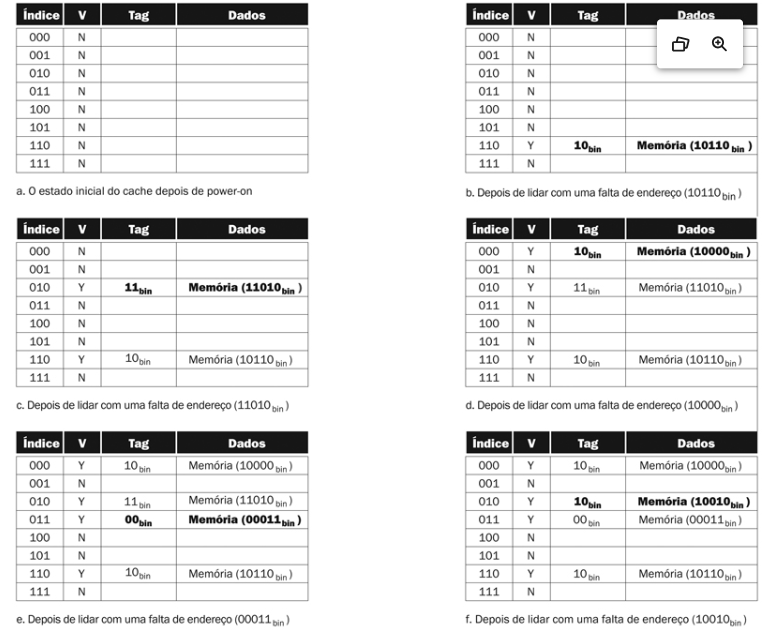
\includegraphics[width=0.8\textwidth]{figuras/localidade_temporal.png}
    \caption{Exemplo de localidade temporal (estados de uma cache)}
    \label{fig:localidade_temporal}
    \fonte{Elaborado pelos autores (2026).}
\end{figure}

\subsection{Localidade espacial}
Blocos maiores exploram a localidade espacial para diminuir as taxas de falhas. Aumentar o tamanho de bloco normalmente diminui a taxa de falhas. A taxa de falhas pode subir posteriormente se o tamanho de bloco se tornar uma fração significativa do tamanho de cache, uma vez que o número de blocos que pode ser armazenado na cache se tornará pequeno e haverá uma grande competição entre esses blocos. Explicando de outra forma: a localidade espacial entre as palavras em um bloco diminui com um bloco muito grande; por conseguinte, os benefícios na taxa de falhas se tornam menores \cite{patterson2017}.

\begin{figure}[H]
    \centering
    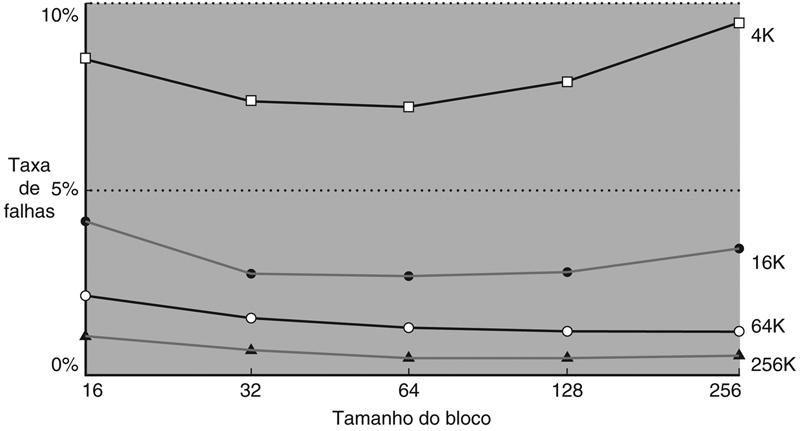
\includegraphics[width=0.7\textwidth]{figuras/localidade_tamanho_bloco.png}
    \caption{Impacto do tamanho do bloco na taxa de falhas}
    \label{fig:localidade_tamanho}
    \fonte{Elaborado pelos autores (2026).}
\end{figure}

\section{Mapeamento}
\subsection{Mapeamento direto}
A maneira mais simples de atribuir um local na cache para cada palavra da memória é atribuir um local na cache baseado no endereço da palavra na memória. Essa estrutura de cache é chamada de mapeamento direto, já que cada local da memória é mapeado diretamente para um local exato na cache.

(Endereço de bloco) módulo (Número de blocos na cache)

Se o número de entradas na cache for uma potência de dois, então, o módulo pode ser calculado simplesmente usando os \(\log_2\) bits menos significativos do endereço \cite{patterson2017}.

\begin{figure}[H]
    \centering
    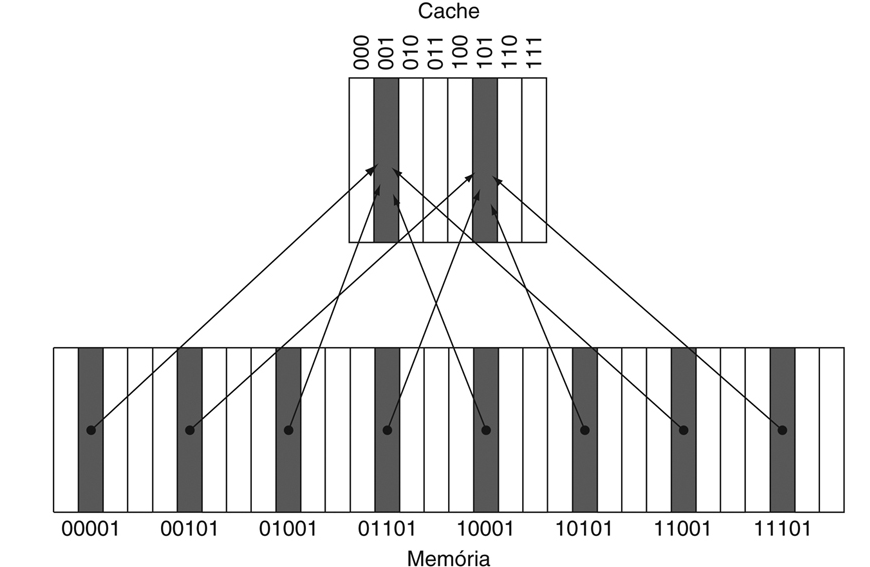
\includegraphics[width=0.8\textwidth]{figuras/mapeamento_direto.png}
    \caption{Exemplo prático de mapeamento direto na memória}
    \label{fig:mapeamento_direto}
    \fonte{Elaborado pelos autores (2026).}
\end{figure}

Como há oito palavras na cache, um endereço X é mapeado para a palavra de cache X, módulo 8. Ou seja, os \(\log_2(8) = 3\) bits menos significativos são usados como o índice da cache. Assim, os endereços \(00001_{bin}\), \(01001_{bin}\), \(10001_{bin}\) e \(11001_{bin}\) são todos mapeados para a entrada \(001_{bin}\) da cache, enquanto os endereços \(00101_{bin}\), \(01101_{bin}\), \(10101_{bin}\) e \(11101_{bin}\) são todos mapeados para a entrada \(101_{bin}\) da cache.

\subsection{Mapeamento totalmente associativo}
Até agora, quando colocamos um bloco na cache, usamos um esquema de posicionamento simples: um bloco só pode entrar exatamente em um local na cache. Como já dissemos, esse esquema é chamado de mapeamento direto porque qualquer endereço de bloco na memória é diretamente mapeado para um único local, no nível superior da hierarquia. Existe, na verdade, toda uma faixa de esquemas para posicionamento de blocos. Em um extremo está o mapeamento direto, em que um bloco só pode ser posicionado exatamente em um local.

No outro extremo está um esquema em que um bloco pode ser posicionado em qualquer local na cache. Para encontrar um determinado bloco em uma cache totalmente associativa, todas as entradas da cache precisam ser pesquisadas. Para tornar a pesquisa possível, ela é feita em paralelo com um comparador associado a cada entrada da cache. Esses comparadores aumentam muito o custo do hardware \cite{patterson2017}.

\subsection{Mapeamento associativo por conjunto}
A faixa intermediária de projetos entre a cache diretamente mapeada e a cache totalmente associativa é chamada de associativa por conjunto. Em uma cache associativa por conjunto, existe um número fixo de locais (pelo menos dois) onde cada bloco pode ser colocado. Um bloco é diretamente mapeado para um conjunto e, então, uma correspondência é pesquisada em todos os blocos no conjunto \cite{patterson2017}.

\begin{figure}[H]
    \centering
    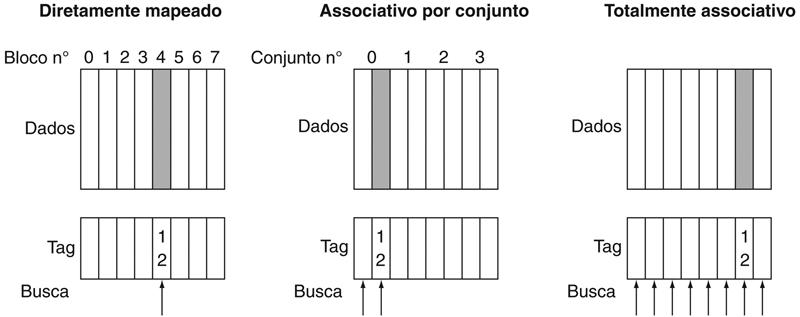
\includegraphics[width=0.9\textwidth]{figuras/tipos_mapeamento.png}
    \caption{Comparação lado a lado: mapeamento direto, associativo e totalmente associativo}
    \label{fig:tipos_mapeamento}
    \fonte{Elaborado pelos autores (2026).}
\end{figure}

\section{Políticas de escrita}
\subsection{Write-through}
A maneira mais simples de manter consistentes a memória principal e a cache é sempre escrever os dados na memória e na cache. Essas escritas levarão muito tempo, talvez mais de 100 ciclos de \textit{clock}. Uma solução é usar um \textit{buffer} de escrita \cite{hennessy2017}.

Com um esquema de \textit{write-through}, toda escrita faz com que os dados sejam escritos na memória principal. Essas escritas levarão muito tempo, talvez mais de 100 ciclos de \textit{clock} de processador, e tornariam o processador consideravelmente mais lento.

Uma solução para esse problema é usar um \textit{buffer} de escrita (ou \textit{write buffer}), que armazena os dados enquanto estão esperando para serem escritos na memória. Após escrever os dados na cache e no \textit{buffer} de dados, o processador pode continuar a execução. Quando uma escrita na memória principal é concluída, a entrada no \textit{buffer} de escrita é liberada.

Se o \textit{buffer} de escrita estiver cheio quando o processador atingir uma escrita, o processador precisará sofrer \textit{stall} até que haja uma posição vazia no \textit{buffer} de escrita. Para reduzir a ocorrência desses \textit{stalls}, os processadores normalmente aumentam a profundidade do \textit{buffer} de escrita para além de uma única entrada.

Considere uma falha em uma cache \textit{write-through}. A estratégia mais comum é alocar um bloco na cache, chamado alocar na escrita. O bloco é apanhado da memória e depois a parte apropriada do bloco é sobrescrita. Uma estratégia alternativa é atualizar a parte do bloco na memória, mas não colocá-la em cache, o que se chama não alocar na escrita. A motivação é que, às vezes, os programas escrevem blocos de dados, como quando o sistema operacional zera uma página de memória. Nesses casos, a busca associada com a falha de escrita inicial pode ser desnecessária.

\subsection{Write-back}
A alternativa é o esquema \textit{write-back}, no qual, quando ocorre uma escrita, o novo valor é escrito apenas no bloco da cache. O bloco modificado é escrito no nível inferior da hierarquia quando ele é substituído. Pode melhorar o desempenho, mas é mais complexo de implementar \cite{hennessy2017}.

Os esquemas \textit{write-back} podem melhorar o desempenho, especialmente quando os processadores podem gerar escritas tão rápido ou mais rápido do que as escritas podem ser tratadas pela memória principal; entretanto, um esquema \textit{write-back} é mais complexo de implementar do que um esquema \textit{write-through}.

Implementar \textit{stores} de modo realmente eficaz em uma cache que usa uma estratégia \textit{write-back} é mais complexo do que em uma cache \textit{write-through}. Em uma cache \textit{write-back}, precisamos escrever o bloco novamente na memória se os dados na cache estiverem modificados e tivermos uma falha de cache.

Em uma cache \textit{write-back}, como não podemos substituir o bloco, os \textit{stores} ou exigem dois ciclos (um ciclo para verificar um acerto seguido de um ciclo para efetivamente realizar a escrita) ou exigem um \textit{buffer} de escrita para conter esses dados na prática, permitindo que a \textit{store} leve apenas um ciclo por meio de um \textit{pipeline} de memória.

Muitas caches \textit{write-back} também incluem \textit{buffers} de escrita usados para reduzir a penalidade de falha quando uma falha substitui um bloco modificado. Em casos como esse, o bloco modificado é movido para um \textit{buffer write-back} associado com a cache enquanto o bloco requisitado é lido da memória. Depois, o \textit{buffer write-back} é escrito novamente na memória.

\section{Taxa de acerto e penalidade de falha}
Essa técnica é baseada na observação de que o processador normalmente precisa de apenas uma palavra do bloco de cada vez. Essa estratégia é a da impaciência: não espere até que o bloco inteiro seja carregado para então enviar a palavra solicitada e reiniciar o processador. Aqui estão duas estratégias específicas:
\begin{itemize}
    \item \textbf{Palavra crítica primeiro:} Solicite primeiro a palavra que falta e envie-a para o processador assim que ela chegar; deixe o processador continuar a execução enquanto preenche o restante das palavras no bloco.
    \item \textbf{Reinício antecipado:} Busque as palavras na ordem normal, mas, assim que a palavra solicitada chegar, envie-a para o processador e deixe que ele continue a execução.
\end{itemize}

Geralmente, essas técnicas só beneficiam projetos com grandes blocos de cache, pois o benefício é baixo, a menos que os blocos sejam grandes. Observe que, normalmente, as caches continuam a satisfazer os acessos a outros blocos enquanto o restante do bloco está sendo preenchido.

Entretanto, dada a proximidade espacial, existe boa chance de que a próxima referência seja para o restante do bloco. Assim como as caches sem bloqueio, a penalidade de falta não é simples de calcular. Quando existe uma segunda solicitação da palavra crítica primeiro, a penalidade de falta efetiva é o tempo não sobreposto da referência até que a segunda parte chegue. Os benefícios da palavra crítica primeiro e de reinício antecipado dependem do tamanho do bloco e da probabilidade de outro acesso à parte do bloco que ainda não foi acessada.

\section{Desafios comuns}
\subsection{Cache thrashing}
A função da memória cache é agilizar a execução de programas, armazenando cópias de blocos de dados da memória principal em uma memória cache mais rápida, embora de menor capacidade. O gráfico na Figura \ref{fig:cache_thrashing} ilustra a taxa de falhas (\textit{miss ratio}) de uma memória cache em função do seu tamanho e associatividade. Quanto menor for o valor da taxa de falhas, melhor será o desempenho da cache. As falhas encontradas em uma memória cache podem ser classificadas em três categorias: falhas compulsórias, por capacidade ou por conflito (também chamadas de 3 Cs) \cite{hennessy2017}.

\begin{itemize}
    \item \textbf{Falhas compulsórias:} São falhas que ocorrem sempre no primeiro acesso a um bloco, já que o bloco nunca foi armazenado na memória cache.
    \item \textbf{Falhas devido à capacidade:} São falhas que ocorrem quando a cache não consegue armazenar todos os blocos necessários à execução de um programa, por não ter capacidade suficiente.
    \item \textbf{Falhas por conflitos ou colisão:} São falhas que ocorrem quando diversos blocos competem pela mesma posição (conjunto) na memória cache. Esse tipo de falha não ocorre em caches totalmente associativas, pois neste caso um bloco pode ser armazenado em qualquer linha da memória cache.
\end{itemize}

\begin{figure}[H]
    \centering
    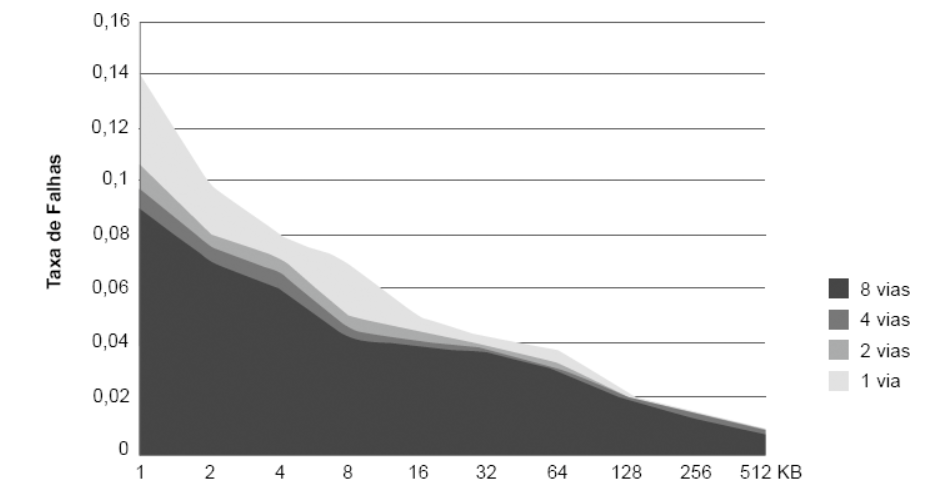
\includegraphics[width=0.8\textwidth]{figuras/localidade_espacial.png}
    \caption{Impacto da associatividade na taxa de falhas}
    \label{fig:cache_thrashing}
    \fonte{Elaborado pelos autores (2026).}
\end{figure}

\subsection{Coerência de cache em múltiplos núcleos}
Nos processadores modernos, com mais de um núcleo, é comum a existência de um terceiro nível de cache (L3), compartilhada por todos os núcleos. O tempo de acesso com acerto a essa cache é da ordem de algumas dezenas de ciclos de relógio. O uso de caches multiníveis é um recurso comum nos modernos processadores, mas que pode resultar na diminuição da taxa de acerto nos níveis mais próximos ao processador, pelo uso de caches com capacidade menor nesses níveis para acompanhar as velocidades crescentes de relógio dos processadores. A arquitetura e o desempenho final de uma memória cache devem ser adequadamente avaliados por meio de simulações, antes da sua implementação física no processador \cite{silva2024}.

\begin{figure}[H]
    \centering
    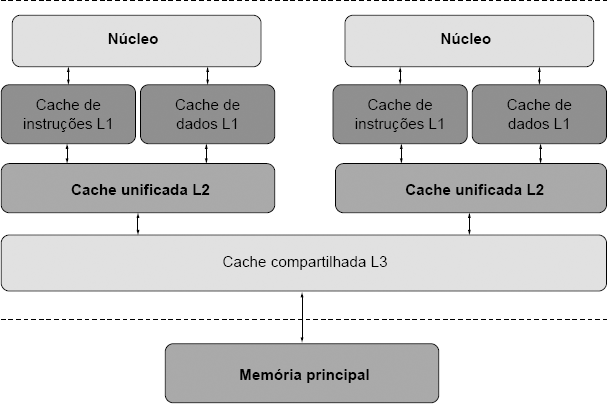
\includegraphics[width=0.8\textwidth]{figuras/hierarquia.png}
    \caption{Caches multiníveis}
    \label{fig:caches_multiniveis}
    \fonte{Elaborado pelos autores (2026).}
\end{figure}

\subsection{Falso compartilhamento}
No início dos tempos a memória cache está vazia, ou seja, não possui nenhuma informação armazenada e todas as suas linhas estão marcadas como inválidas. As instruções e dados vão sendo então gradativamente copiados dos níveis inferiores, como a memória principal e secundária, para a memória cache, à medida que são utilizados pelo processador. Na realidade, o processador inicia a busca das instruções ou dos dados na suposição de que estejam armazenados na memória cache. Se forem encontrados na memória cache (houve um acerto), a informação desejada é transferida para o processador. Mas se os dados ou a instrução não estiverem na memória cache (houve uma falha), então o processador aguarda, enquanto a instrução/dados desejados são copiados para a memória cache e depois transferidos para o processador.

Durante a busca da informação que está faltando na cache, em vez de trazer somente a instrução ou dados solicitados pelo processador, um bloco inteiro é copiado da memória principal e armazenado em uma linha da cache, que então é marcada como válida. O objetivo é minimizar a taxa de falhas nos próximos acessos, seguindo o princípio da localidade espacial. O tamanho de um bloco é um parâmetro de projeto nas memórias caches, tamanhos usuais são 32, 64 e 128 bytes. Note que um bloco trazido da memória principal recebe o nome de linha quando armazenado na memória cache, sendo, portanto, de mesmo tamanho \cite{silva2024}.

\section{Técnicas de otimização}
Essas otimizações aumentam a largura de banda da cache seja pelo \textit{pipelining} do acesso à cache ou pela ampliação da cache com múltiplos bancos, permitindo múltiplos acessos por ciclo de \textit{clock}; essas otimizações estão associadas às abordagens \textit{superpipelined} e superescalar para aumentar o \textit{throughput} de instrução. Elas visam principalmente a cache L1, onde a largura de banda de acesso restringe o \textit{throughput} de instrução.

O \textit{pipelining} L1 permite um ciclo de \textit{clock} mais alto, ao custo de uma maior latência. O \textit{pipelining} da cache de instruções efetivamente aumenta o número de estágios do \textit{pipeline}, levando a uma penalidade maior nos desvios mal previstos. De modo correspondente, o \textit{pipelining} da cache de dados leva a mais ciclos de \textit{clock} entre a emissão do \textit{load} e o uso dos dados.

Para lidar com múltiplos acessos à cache de dados por \textit{clock}, podemos dividir a cache em bancos independentes, cada um suportando um acesso independente. Os bancos foram originalmente usados para melhorar o desempenho da memória principal e agora são usados dentro de chips DRAM modernos, bem como com caches. O Intel Core i7 contém quatro bancos na cache L1 (para admitir até 2 acessos de memória por \textit{clock}) \cite{hennessy2019}.

Uma cache sem bloqueio ou cache sem travamento aumenta os benefícios em potencial de tal esquema, permitindo que a cache de dados continue a fornecer acertos de cache durante uma falta. Essa otimização de ``acerto sob falta'' reduz a penalidade de falta efetiva, sendo útil durante uma falta, em vez de ignorar as solicitações do processador. Uma opção sutil e complexa é que a cache pode reduzir ainda mais a penalidade de falta efetiva se puder sobrepor múltiplas faltas: uma otimização ``acerto sob múltiplas faltas'' ou ``falta sob falta''. A segunda opção só será benéfica se o sistema de memória puder atender a múltiplas faltas; a maior parte dos processadores de alto desempenho (como os processadores Intel Core) geralmente suporta ambos, enquanto muitos dos processadores de baixo nível oferecem somente suporte limitado sem bloqueio na cache L2 \cite{hennessy2019}.

Até aqui, nossas técnicas têm exigido a mudança do hardware. Essa próxima técnica reduz as taxas de falta sem quaisquer mudanças no hardware. Essa redução mágica vem do software otimizado a solução favorita do projetista de hardware! A diferença de desempenho cada vez maior entre os processadores e a memória principal tem inspirado os projetistas de compiladores a investigar a hierarquia de memória para ver se as otimizações em tempo de compilação podem melhorar o desempenho. Mais uma vez, a pesquisa está dividida entre as melhorias nas faltas de instrução e as melhorias nas faltas de dados. As otimizações apresentadas a seguir são encontradas em muitos compiladores modernos.

Em vez de operar sobre linhas ou colunas inteiras de um \textit{array}, os algoritmos bloqueados operam sobre submatrizes ou blocos. O objetivo é maximizar os acessos aos dados carregados na cache antes que eles sejam substituídos \cite{hennessy2019}.

As caches sem bloqueio reduzem efetivamente a penalidade de falta, sobrepondo a execução com o acesso à memória. Outra técnica é fazer a pré-busca (\textit{prefetch}) dos itens antes que o processador os solicite. Tanto as instruções quanto os dados podem ter sua busca antecipada, seja diretamente nas caches, seja diretamente em um buffer externo, que pode ser acessado mais rapidamente do que a memória principal.

Frequentemente, a pré-busca de instrução é feita no hardware fora da cache. Em geral, o processador apanha dois blocos em uma falta: o bloco solicitado e o próximo bloco consecutivo. O bloco solicitado é colocado na cache de instruções, e o bloco cuja busca foi antecipada é colocado no buffer do fluxo de instruções. Se o bloco solicitado estiver presente no buffer do fluxo de instruções, a solicitação de cache original será cancelada, o bloco será lido do buffer de fluxo e a próxima solicitação de pré-busca será emitida \cite{hennessy2019}.